\documentclass[../notes.tex]{subfiles}

\pagestyle{main}
\renewcommand{\chaptermark}[1]{\markboth{\chaptername\ \thechapter\ (#1)}{}}
\setcounter{chapter}{6}

\begin{document}




\chapter{Gas-Phase Product Molecule Analysis and Intro to Lattices}
\section{Directional Scattering of the Product Molecule}
\begin{itemize}
    \item \marginnote{5/9:}The velocity and angular distribution of the products of a reactive collision.
    \begin{itemize}
        \item We have that
        \begin{align*}
            E_\text{trans}'+E_\text{vib}' &= E_\text{trans}+E_\text{vib}-[D_e(\ce{D2})-D_e(\ce{DF})]\\
            &= \SI{7.62}{\kilo\joule\per\mole}+\SI{17.9}{\kilo\joule\per\mole}+\SI{140}{\kilo\joule\per\mole}\\
            &= \SI{166}{\kilo\joule\per\mole}
        \end{align*}
        \item Additionally, we know that
        \begin{equation*}
            E_\text{trans}'+E_\text{vib}' = \frac{1}{2}\mu'u_r'^2+(\SI{34.8}{\kilo\joule\per\mole})\left( v+\frac{1}{2} \right)
            = \SI{166}{\kilo\joule\per\mole}
        \end{equation*}
        \item The relationship between the vibrational quantum number, the relative speed of the products, and the speed of \ce{DF} relative to the center of mass has been tabulated.
    \end{itemize}
    \item A contour map of the angular and speed distributions for the product molecule.
    \begin{itemize}
        \item The contour plot.
        \begin{itemize}
            \item The center of mass is fixed at the origin.
            \item The dashed circles correspond to the maximum relative speeds a \ce{DF} molecule can have for the indicated vibrational state.
            \item The product molecules preferentially scatter back in the direction of the incident fluorine atom, a scattering angle of $\theta=\ang{180}$.
            \item The arrows at the bottom of the figure show the direction with which each reactant molecule approaches the other.
        \end{itemize}
        \item Another picture is provided, illustrating the atom-molecule reaction \ce{F + D2} in which $\theta=\ang{0}$ and $\theta=\ang{180}$.
        \item The influence of rotation.
        \begin{itemize}
            \item Large numbers of product molecules have speeds between the dashed circles.
            \item The dash circles correspond to the case where there is internal energy only in the vibrational states of the molecule, in which case the rotational energy corresponding to these circles is $E_\text{rot}=0$ with $J=0$.
            \item If \ce{DF} is produced in an excited rotational state, we would expect to observe a speed that has a value intermediate between two fo the dashed circles.
        \end{itemize}
    \end{itemize}
    \item Not all gas-phase chemical reactions are rebound reactions.
    \begin{itemize}
        \item Consider the reaction
        \begin{equation*}
            \ce{K(g) + I2(g) -> KI(g) + I(g)}
        \end{equation*}
        \begin{itemize}
            \item The product diatomic molecule in this case (\ce{KI}) is preferentially scattered in the forward direction along the direction of the incident \ce{K} atom.
        \end{itemize}
        \item Consider the reaction
        \begin{equation*}
            \ce{O(g) + Br2(g)} \Longrightarrow \ce{BrO(g) + Br(g)}
        \end{equation*}
        \begin{itemize}
            \item The product molecule \ce{BrO} is forward and back scattered with equal intensity.
        \end{itemize}
        \item Both of these observations can be read off of the contour maps of the two reactions.
    \end{itemize}
\end{itemize}



\section{Potential Energy Surfaces}
\begin{itemize}
    \item \marginnote{5/11:}The velocity and angular distribution of the products of a reactive collision.
    \begin{figure}[h!]
        \centering
        \begin{tikzpicture}
            \footnotesize
            \draw [dashed] (-5.5,0) -- (-0.18,0) (5.5,0) -- (0.18,0);
    
            \draw
                (-4,0) ellipse (7mm and 1.5cm) node[above=2cm,align=center]{Approaching\\reactant}
                (4,0) ellipse (1.05cm and 2.25cm) node[above=2.75cm,align=center]{Leaving\\product}
            ;
            \draw
                (-4,0) ++(145:1.5) ++(0.65,0) coordinate(A) -- (-4,0)
                (-4,0) ++(20:1.5) ++(-0.75,0) coordinate (A') -- (-4,0)
                ($(-4,0)!0.3!(A)$) arc[start angle=150,end angle=18,x radius=2.1mm,y radius=4.5mm]
                ($(-4,0)!0.25!(A')$) -- ++(0.25,0) -- (-3.75,0)
            ;
            \node at (-4,0.65) {$\phi$};
            \draw
                (4,0) ++(145:2.25) ++(0.98,0) coordinate(C) -- (4,0)
                (4,0) ++(20:2.25) ++(-1.13,0) coordinate (C') -- (4,0)
                ($(4,0)!0.2!(C)$) arc[start angle=150,end angle=18,x radius=2.1mm,y radius=4.5mm]
                ($(4,0)!0.17!(C')$) -- ++(0.25,0) -- (4.25,0)
            ;
            \node at (4,0.65) {$\phi$};
    
            \draw [semithick,-latex] (A) -- node[above]{$\mathbf{u}_r$} (A -| 0,0) -- node[above]{$\mathbf{u}_r'$} ($(A -| 0,0)!0.84!(C)$);
            \draw (A -| -0.45,0) arc[start angle=180,end angle=8,radius=4.5mm];
            \node [fill=white,inner sep=1.5pt] at ([yshift=4.5mm]A -| 0,0) {$\theta$};
    
            \draw [<->,shorten <=1pt,shorten >=1pt] (-2,0 |- A) -- node[right]{$b$} (-2,0);
    
            \begin{scope}[on background layer]
                \fill [ball color=rex] (0,0) circle (1cm) node{\ce{B}};
                \fill [ball color=blx] (A) circle (5mm) node[left]{\ce{A}};
                \fill [ball color=blx] (C) circle (5mm);
            \end{scope}
        \end{tikzpicture}
        \caption{Velocity and angular distributions of the products.}
        \label{fig:velocityAngleDist}
    \end{figure}
    \begin{itemize}
        \item For a fixed value of the impact parameter $b$, the reactants and products take on all possible angles $\phi$ with equal probability, thereby forming a cone around the relative velocity vector $\mathbf{u}_r$.
        \item The angle $\theta$, however, depends on the dynamics of the reaction and must be determined experimentally.
    \end{itemize}
    \item The potential energy of a polyatomic molecule depends on more than one variable.
    \begin{itemize}
        \item \ce{D2}.
        \begin{itemize}
            \item Consider the potential energy curve of \ce{D2}. The zero of energy is defined to be that of the two separated atoms. The minimum of the potential energy curve corresponds to the equilibrium bond length of the \ce{D2} molecule.
        \end{itemize}
        \item \ce{H2O}.
        \begin{itemize}
            \item The potential energy of a water molecule is a function of the three parameters $r_{\ce{O-H_A}}$, $r_{\ce{O-H_B}}$, and $\alpha$ (two bond lengths and the interbond angle). In an equation,
            \begin{equation*}
                V = V(r_{\ce{O-H_A}},r_{\ce{O-H_B}},\alpha)
            \end{equation*}
            \item A plot of the complete potential energy surface of a water molecule therefore requires four axes.
        \end{itemize}
    \end{itemize}
    \item The potential energy of a chemical reaction depends on more than one variable.
    \begin{figure}[H]
        \centering
        \footnotesize
        \begin{subfigure}[b]{0.3\linewidth}
            \centering
            \begin{tikzpicture}
                \node (DA) at (0,0)   {\ce{D_A}};
                \node (DB) at (1.3,0) {\ce{D_B}};
                \node (F)  at (180:2) {\ce{F}};
    
                \draw [semithick,dashed] (F)  -- node[above]{$\beta=\ang{180}$} (DA);
                \draw [semithick] (DA) -- (DB);
            \end{tikzpicture}
            \caption{Linear.}
            \label{fig:FD2attackAnglea}
        \end{subfigure}
        \begin{subfigure}[b]{0.3\linewidth}
            \centering
            \begin{tikzpicture}
                \node (DA) at (0,0)   {\ce{D_A}};
                \node (DB) at (1.3,0) {\ce{D_B}};
                \node (F)  at (135:2) {\ce{F}};
    
                \draw [semithick,dashed] (F)  -- node[above right]{$\beta=\ang{180}$} (DA);
                \draw [semithick] (DA) -- (DB);
            \end{tikzpicture}
            \caption{Bent.}
            \label{fig:FD2attackAngleb}
        \end{subfigure}
        \begin{subfigure}[b]{0.3\linewidth}
            \centering
            \begin{tikzpicture}
                \node (DA) at (0,0)   {\ce{D_A}};
                \node (DB) at (1.3,0) {\ce{D_B}};
                \node (F)  at (90:2) {\ce{F}};
    
                \draw [semithick,dashed] (F)  -- node[right]{$\beta=\ang{180}$} (DA);
                \draw [semithick] (DA) -- (DB);
            \end{tikzpicture}
            \caption{Perpendicular.}
            \label{fig:FD2attackAnglec}
        \end{subfigure}
        \caption{Angle of attack in \ce{F + D2}.}
        \label{fig:FD2attackAngle}
    \end{figure}
    \begin{itemize}
        \item Consider, once again, the reaction
        \begin{equation*}
            \ce{F(g) + D_AD_B(g)} \Longrightarrow \ce{D_AF(g) + D_B(g)}
        \end{equation*}
        \item When the reactants are at infinite separation, there are no attractive or repulsive forces between the fluorine atom and the \ce{D2} molecule, so the potential energy surface for the reaction is the same as that for an isolated \ce{D2} molecule.
        \item Likewise, when the products are at infinite separation, the potential-energy surface for the reaction is the same as the for the isolated \ce{DF} molecule.
        \item As the reaction occurs, however, the distance between the fluroine atom and \ce{D_A} decreases and the distance between \ce{D_A} and \ce{D_B} increases, and the potential energy depends on both distances.
        \item The potential energy also depends on the angle at which the \ce{F} atom approaches the \ce{D2} molecule.
    \end{itemize}
    \item As with the angular and speed distributions, we can draw an energy contour map for the reaction.
    \begin{itemize}
        \item The zero of energy is defined as the infinitely separated reactants. Point B is the location of the transition state of the reaction.
    \end{itemize}
    \item Tian does a brief summary of Chapter 30.
\end{itemize}



\section{Lattice Structure}
\begin{itemize}
    \item \marginnote{5/13:}The unit cell is the fundamental building block of a crystal.
    \begin{itemize}
        \item We can think of a crystal as a two- or three-dimensional lattice.
        \item Either way, we can identify blocks in the lattice that form a regularly repeating structure.
    \end{itemize}
    \item \textbf{Face-centered cubic} (unit cell): The following unit cell. \emph{Also known as} \textbf{FCC}, \textbf{cubic close-packing}. \emph{Structure}
    \begin{figure}[H]
        \centering
        \begin{subfigure}[b]{0.2\linewidth}
            \centering
            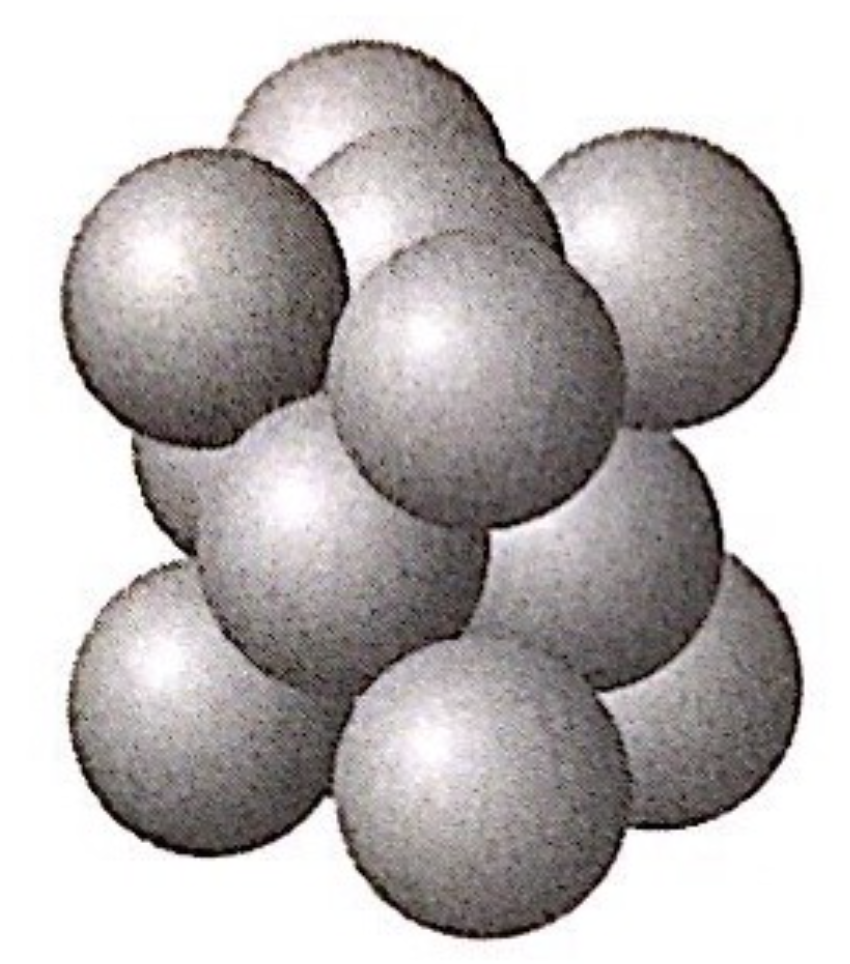
\includegraphics[width=0.6\linewidth]{../ExtFiles/FCCunitCella.png}
            \caption{Atomic picture.}
            \label{fig:FCCunitCella}
        \end{subfigure}
        \begin{subfigure}[b]{0.2\linewidth}
            \centering
            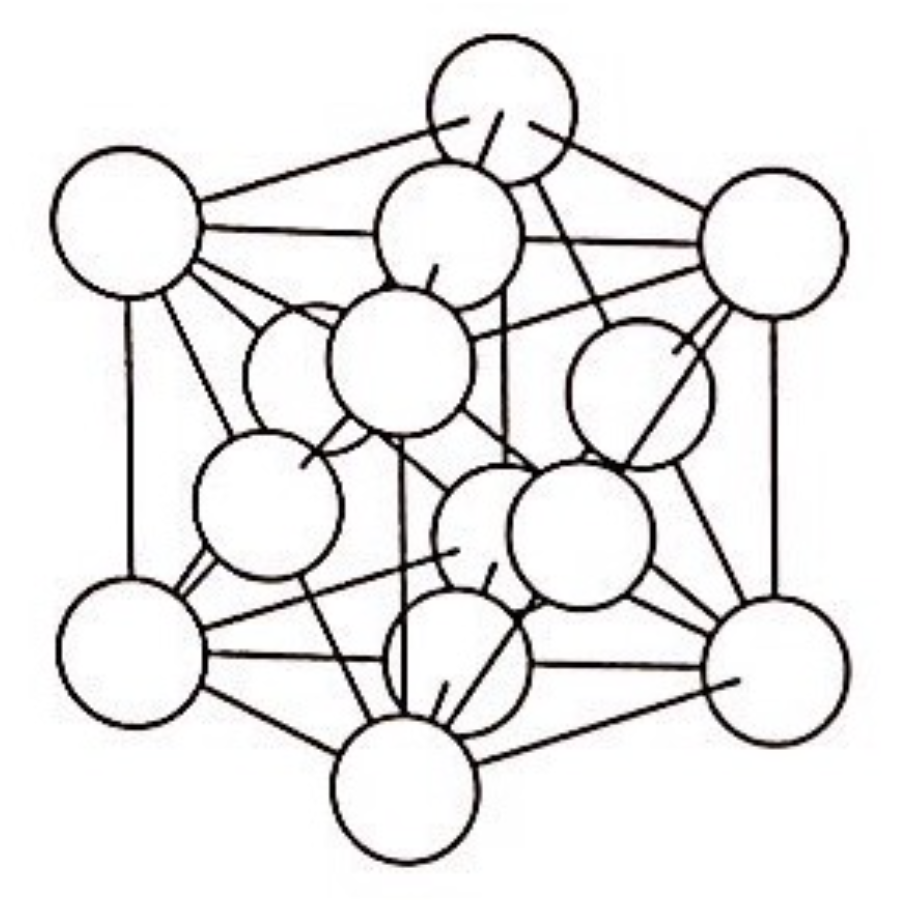
\includegraphics[width=0.7\linewidth]{../ExtFiles/FCCunitCellb.png}
            \caption{Lattice picture.}
            \label{fig:FCCunitCellb}
        \end{subfigure}
        \begin{subfigure}[b]{0.2\linewidth}
            \centering
            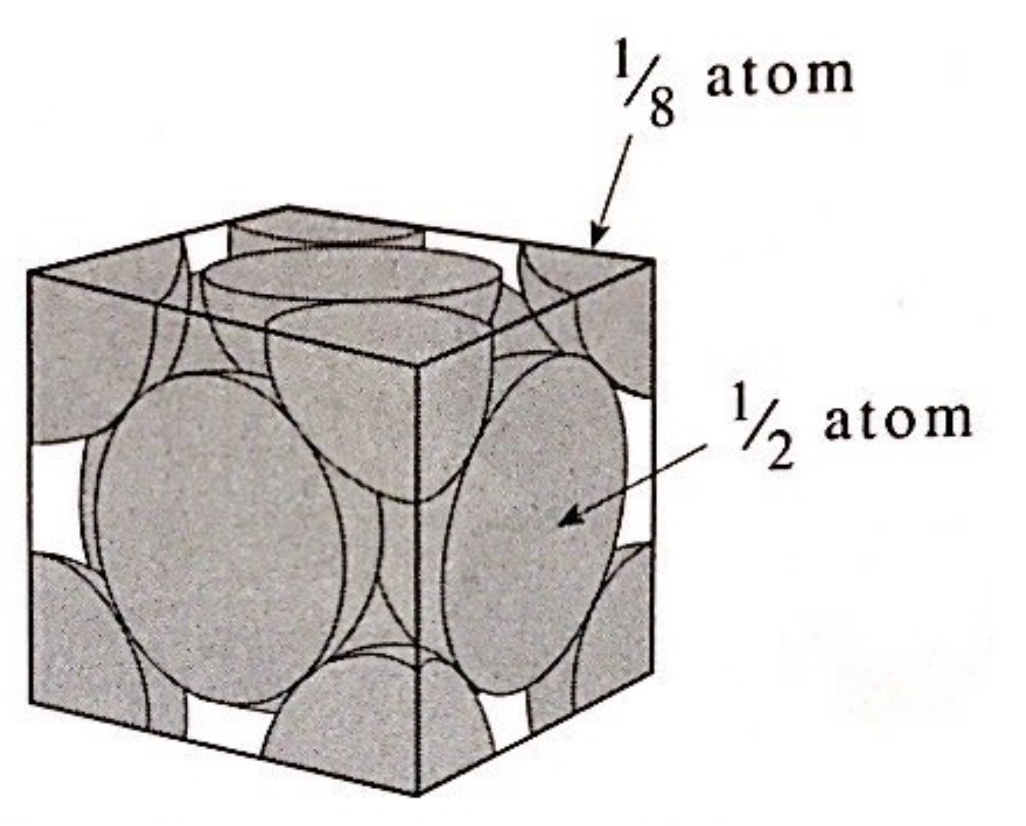
\includegraphics[width=1.0\linewidth]{../ExtFiles/FCCunitCellc.png}
            \caption{Unit cell.}
            \label{fig:FCCunitCellc}
        \end{subfigure}
        \caption{Face-centered cubic unit cell.}
        \label{fig:FCCunitCell}
    \end{figure}
    \begin{itemize}
        \item Figure \ref{fig:FCCunitCella} shows the set of atoms that contribute to a unit cell of the crystal. The unit cell, itself, is a cube however (see Figure \ref{fig:FCCunitCellc}).
        \item Figure \ref{fig:FCCunitCellb} shows the unit cell for a three-dimensional lattice model of copper, where each point of the crystal is associated with a lattice point.
        \item Figure \ref{fig:FCCunitCellc} shows the fractions of each copper atom shown in Figure \ref{fig:FCCunitCella} that contribute to the unit cell of the crystal.
        \item There are four atoms per unit cell (six half-atoms and eight eighth-atoms).
        \item Example: The packing of copper atoms in a copper crystal gives a face-centered cubic unit cell.
    \end{itemize}
    \item \textbf{Body-centered cubic} (unit cell): The following unit cell. \emph{Also known as} \textbf{BCC}. \emph{Structure}
    \begin{figure}[h!]
        \centering
        \begin{subfigure}[b]{0.2\linewidth}
            \centering
            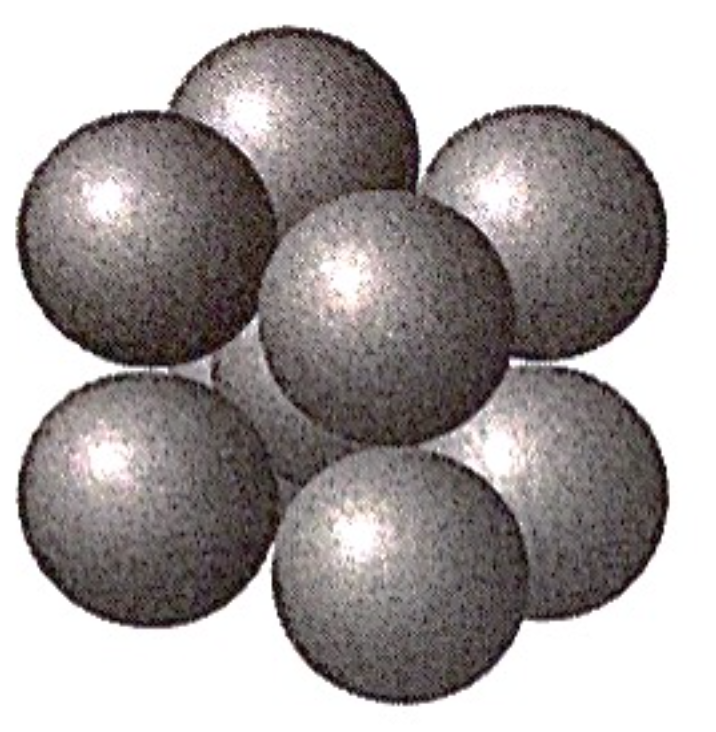
\includegraphics[width=0.6\linewidth]{../ExtFiles/BCCunitCella.png}
            \caption{Atomic picture.}
            \label{fig:BCCunitCella}
        \end{subfigure}
        \begin{subfigure}[b]{0.2\linewidth}
            \centering
            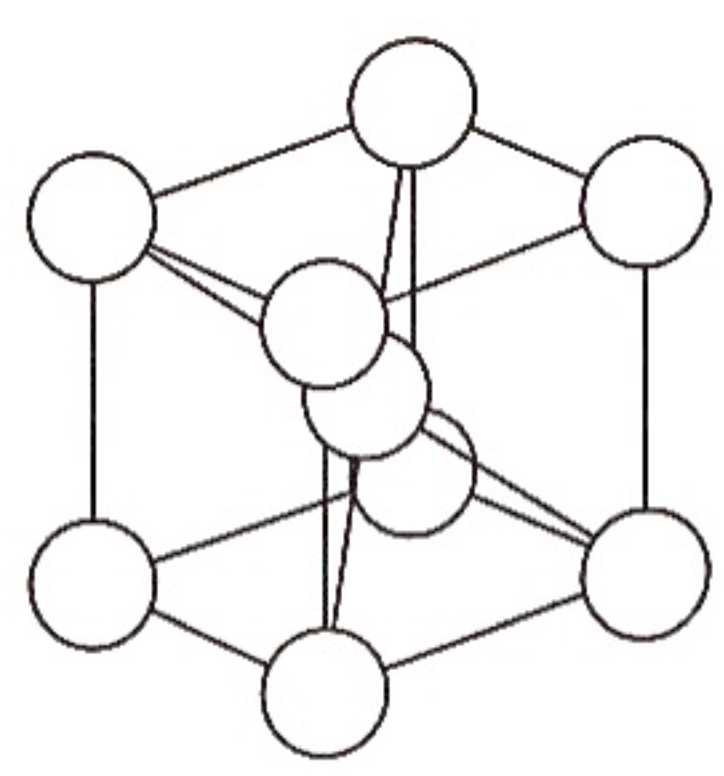
\includegraphics[width=0.65\linewidth]{../ExtFiles/BCCunitCellb.png}
            \caption{Lattice picture.}
            \label{fig:BCCunitCellb}
        \end{subfigure}
        \begin{subfigure}[b]{0.2\linewidth}
            \centering
            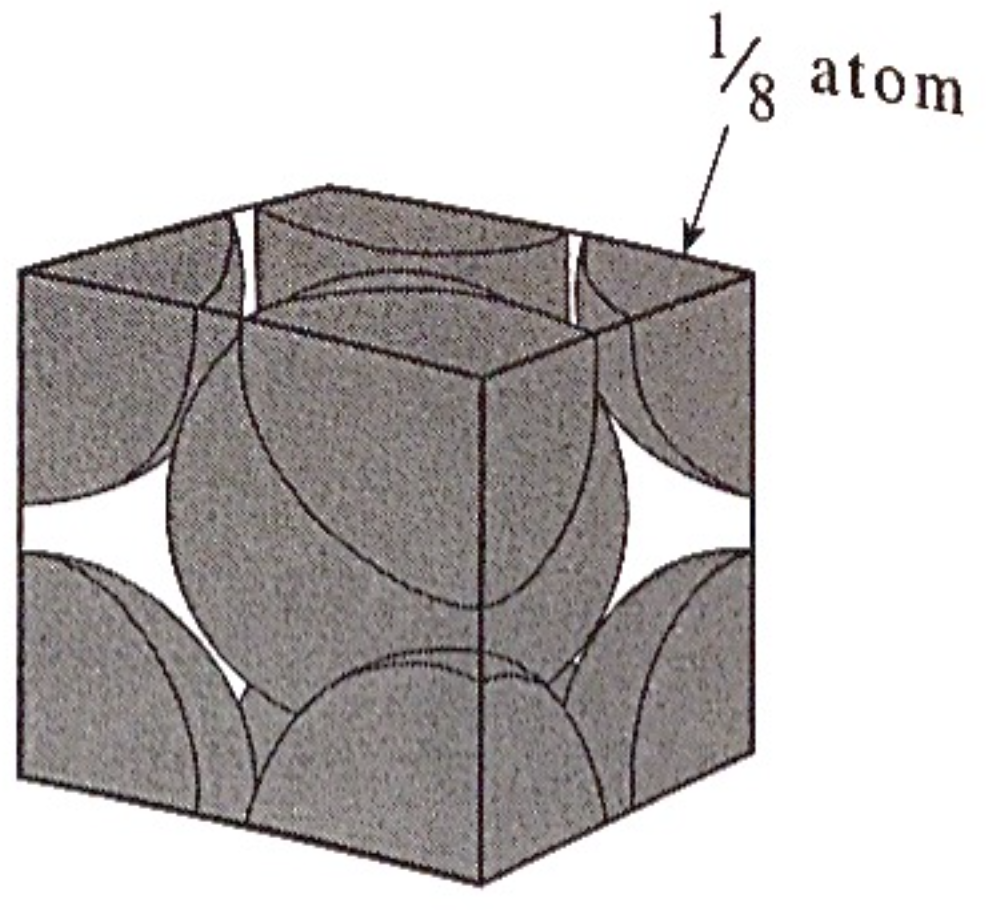
\includegraphics[width=0.85\linewidth]{../ExtFiles/BCCunitCellc.png}
            \caption{Unit cell.}
            \label{fig:BCCunitCellc}
        \end{subfigure}
        \caption{Body-centered cubic unit cell.}
        \label{fig:BCCunitCell}
    \end{figure}
    \begin{itemize}
        \item There are two atoms per unit cell.
        \item Example: The packing of potassium atoms in a crystal.
    \end{itemize}
    \item \textbf{Primitive cubic} (unit cell): The following unit cell. \emph{Also known as} \textbf{simple cubic}. \emph{Structure}
    \begin{figure}[h!]
        \centering
        \begin{subfigure}[b]{0.2\linewidth}
            \centering
            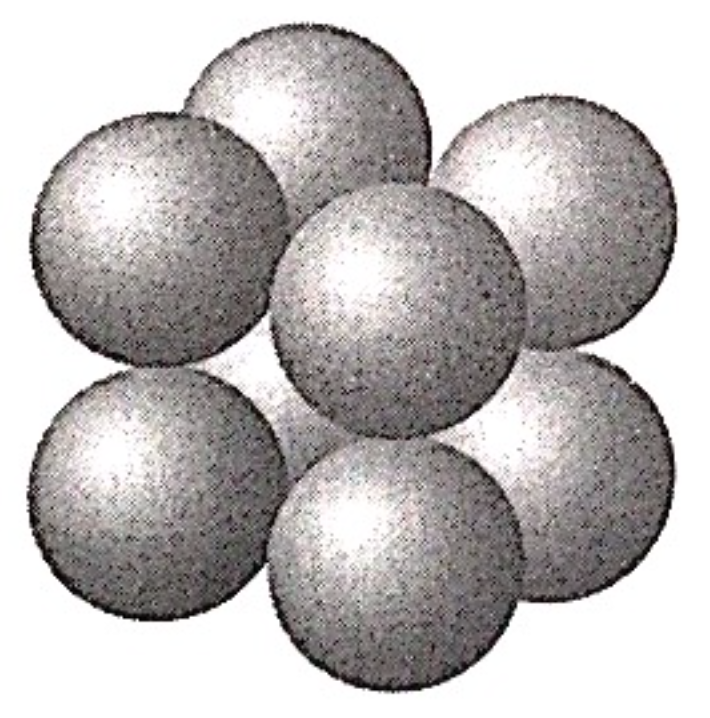
\includegraphics[width=0.6\linewidth]{../ExtFiles/PCunitCella.png}
            \caption{Atomic picture.}
            \label{fig:PCunitCella}
        \end{subfigure}
        \begin{subfigure}[b]{0.2\linewidth}
            \centering
            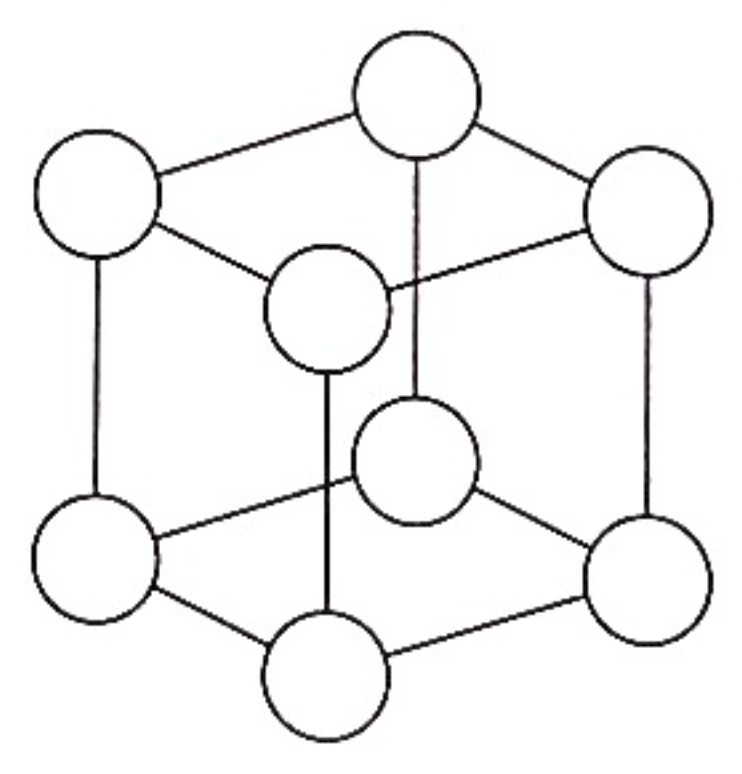
\includegraphics[width=0.65\linewidth]{../ExtFiles/PCunitCellb.png}
            \caption{Lattice picture.}
            \label{fig:PCunitCellb}
        \end{subfigure}
        \begin{subfigure}[b]{0.2\linewidth}
            \centering
            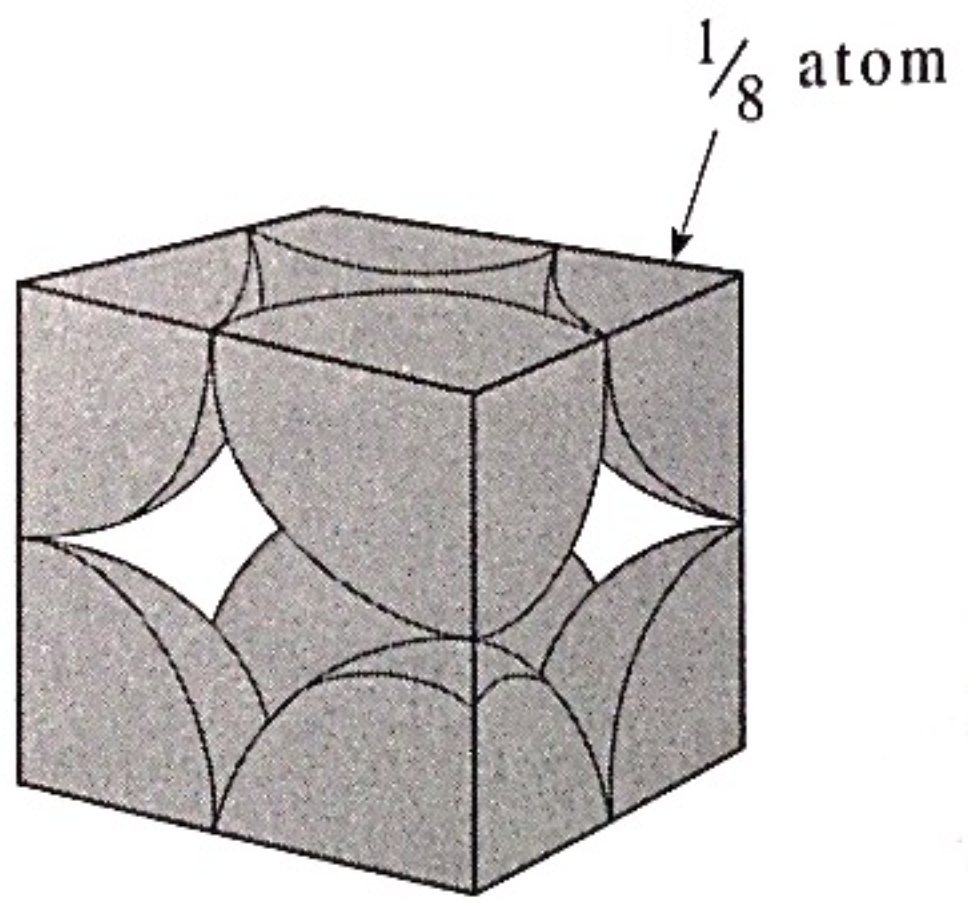
\includegraphics[width=0.85\linewidth]{../ExtFiles/PCunitCellc.png}
            \caption{Unit cell.}
            \label{fig:PCunitCellc}
        \end{subfigure}
        \caption{Body-centered cubic unit cell.}
        \label{fig:PCunitCell}
    \end{figure}
    \begin{itemize}
        \item There is one atom per unit cell.
        \item Example: The packing of polonium atoms in a crystal.
    \end{itemize}
    \item \textbf{Unit cell}: The simplest repeating unit in the crystal. \emph{Structure}
    \begin{figure}[H]
        \centering
        \begin{tikzpicture}[scale=2,z={(4.85mm,3.85mm)}]
            \footnotesize
            \draw
                (0,0,0) coordinate (O) -- node[below]{$a$} (1,0,0) coordinate (a) -- node[below right=-1pt]{$b$} (1,0,1) -- (0,0,1) coordinate (b) -- cycle
                (0.4,1.2,0) coordinate (c) -- ++(1,0,0) -- ++(0,0,1) -- ++(-1,0,0) -- cycle
                (O) -- (c)
                (a) -- ($(a)+(c)$)
                (b) -- ($(b)+(c)$)
                ($(a)+(b)$) -- node[right]{$c$} ($(a)+(b)+(c)$)
            ;
    
            \pic [draw,angle eccentricity=1.3,pic text={$\alpha$}] {angle=b--O--c};
            \pic [draw,angle radius=1cm] {angle=a--O--c};
            \node [fill=white,inner sep=1pt] at (20:0.5) {$\beta$};
            \pic [draw,angle radius=4mm,angle eccentricity=1.3,pic text={$\gamma$}] {angle=a--O--b};
    
            \draw [-stealth] ([xshift=-1cm]O) -- ([xshift=-1cm]$(O)!0.5!(a)$)  node[right]{\textbf{a}};
            \draw [-stealth] ([xshift=-1cm]O) -- ([xshift=-1cm]$(O)!0.65!(b)$) node[above right=-1pt]{\textbf{b}};
            \draw [-stealth] ([xshift=-1cm]O) -- ([xshift=-1cm]$(O)!0.5!(c)$)  node[right]{\textbf{c}};
        \end{tikzpicture}
        \caption{Unit cell.}
        \label{fig:unitCell}
    \end{figure}
    \begin{itemize}
        \item Opposite faces of a unit cell are parallel.
        \item The edge of the unit cell connects equivalent points.
        \item Unit cells all have the same general shape.
        \begin{itemize}
            \item We take the bottom left corner of the unit cell to be the origin of the \textbf{a}, \textbf{b}, \textbf{c} coordinate system.
            \item The unit cell is defined by the distances $a$, $b$, and $c$ (which give its length along the \textbf{a}, \textbf{b}, and \textbf{c} axes, respectively) and the angles $\alpha$, $\beta$, and $\gamma$ (which lie between the three pairs of axes).
        \end{itemize}
        \item Note that henceforth unless stated otherwise, the \textbf{a} axis points to the right, the \textbf{b} axis points back, and the \textbf{c} axis points up, as in Figure \ref{fig:unitCell}.
    \end{itemize}
    \item Tian gives examples of unit cells for crystals containing more than one atom as well as what kinds of crystals take these structures.
    \item \textbf{Bravais lattices}: The fourteen distinct unit cells necessary to generate all possible crystal lattices.
    \begin{itemize}
        \item The French physicist August Bravais proved that only the Bravais lattices are needed to generate all possible structures.
    \end{itemize}
    \item We can interpret the points in the unit cell as atoms or molecules. For example, crystalline \ce{C_{60}} forms a face-centered cubic unit cell.
    \item \textbf{Miller indices}: The three indices that we use to specify parallel planes through a crystal lattice. \emph{Denoted by} $\bm{h}$, $\bm{k}$, $\bm{l}$. \emph{Given by}
    \begin{align*}
        h &= \frac{a}{a'}&
        k &= \frac{b}{b'}&
        l &= \frac{c}{c'}
    \end{align*}
    where the plane in question intersects the \textbf{a}, \textbf{b}, and \textbf{c} axes of the unit cell at points $a'$, $b'$, and $c'$, respectively.
    \item Three basic types of planes.
    \begin{figure}[h!]
        \centering
        \begin{subfigure}[b]{0.2\linewidth}
            \centering
            \begin{tikzpicture}[z={(4.85mm,7mm)},line join=round]
                \draw [semithick] (0,0,0) -- (2,0,0) -- (2,0,1) -- (0,0,1) -- cycle;
                \filldraw [semithick,fill=rey]
                    (0,1,0) -- (0,0,0) -- (0,0,1) -- (0,1,1)
                    (1,1,0) -- (1,0,0) -- (1,0,1) -- (1,1,1)
                    (2,1,0) -- (2,0,0) -- (2,0,1) -- (2,1,1)
                ;
                \draw [semithick]
                    (0,1,0) -- (2,1,0) -- (2,1,1) -- (0,1,1) -- cycle
                    (1,1,0) -- (1,1,1)
                ;
            \end{tikzpicture}
            \caption{$100$ planes.}
            \label{fig:basicPlanesa}
        \end{subfigure}
        \begin{subfigure}[b]{0.2\linewidth}
            \centering
            \begin{tikzpicture}[z={(4.85mm,7mm)},line join=round]
                \draw [semithick] (0,0,0) -- (2,0,0) -- (2,0,1) -- (0,0,1) -- cycle;
                \draw [semithick]
                    (0,1,0) -- (0,0,0) -- (0,0,1) -- (0,1,1)
                    (1,1,0) -- (1,0,0) -- (1,0,1) -- (1,1,1)
                    (2,1,0) -- (2,0,0) -- (2,0,1) -- (2,1,1)
                ;
                \filldraw [semithick,fill=rey]
                    (1,0,0) -- (0,0,1) -- (0,1,1) -- (1,1,0) -- cycle
                    (2,0,0) -- (1,0,1) -- (1,1,1) -- (2,1,0) -- cycle
                ;
                \draw [semithick]
                    (0,1,0) -- (2,1,0) -- (2,1,1) -- (0,1,1) -- cycle
                    (1,1,0) -- (1,1,1)
                ;
            \end{tikzpicture}
            \caption{$110$ planes.}
            \label{fig:basicPlanesb}
        \end{subfigure}
        \begin{subfigure}[b]{0.2\linewidth}
            \centering
            \begin{tikzpicture}[z={(4.85mm,7mm)},line join=round]
                \draw [semithick] (0,0,0) -- (2,0,0) -- (2,0,1) -- (0,0,1) -- cycle;
                \draw [semithick]
                    (0,1,0) -- (0,0,0) -- (0,0,1) -- (0,1,1)
                    (1,1,0) -- (1,0,0) -- (1,0,1) -- (1,1,1)
                    (2,1,0) -- (2,0,0) -- (2,0,1) -- (2,1,1)
                ;
                \filldraw [semithick,fill=rey]
                    (1,0,0) -- (0,0,1) -- (0,1,0) -- cycle
                    (2,0,0) -- (1,0,1) -- (0,1,1) -- (1,1,0) -- cycle
                    (2,0,1) -- (2,1,0) -- (1,1,1) -- cycle
                ;
                \draw [semithick]
                    (0,1,0) -- (2,1,0) -- (2,1,1) -- (0,1,1) -- cycle
                    (1,1,0) -- (1,1,1)
                ;
            \end{tikzpicture}
            \caption{$111$ planes.}
            \label{fig:basicPlanesc}
        \end{subfigure}
        \caption{Basic lattice planes.}
        \label{fig:basicPlanes}
    \end{figure}
    \begin{itemize}
        \item Why are they called as such? Esp. where are the zeros coming from?
    \end{itemize}
    \item Denoting more complicated types of planes.
    \begin{figure}[H]
        \centering
        \begin{subfigure}[b]{0.2\linewidth}
            \centering
            \begin{tikzpicture}[z={(3.85mm,6mm)},line join=round,yscale=1.2]
                \path (0,0,0) -- (0,-1,0);
                \draw [semithick] (0,0,0) -- (1,0,0) -- (1,0,1) -- (0,0,1) -- cycle;
                \draw [semithick]
                    (0,1,0) -- (0,0,0) -- (0,0,1) -- (0,1,1)
                    (1,1,0) -- (1,0,0) -- (1,0,1) -- (1,1,1)
                ;
                \filldraw [semithick,fill=rey] (1,0,0.5) -- (0.5,0,1) -- (0.5,1,1) -- (1,1,0.5) -- cycle;
                \filldraw [semithick,fill=rey] (1,0,0) -- (0,0,1) -- (0,1,1) -- (1,1,0) -- cycle;
                \filldraw [semithick,fill=rex] (0.5,0,0) -- (0,0,0.5) -- (0,1,0.5) -- (0.5,1,0) -- cycle;
                \draw [semithick] (0,1,0) -- (1,1,0) -- (1,1,1) -- (0,1,1) -- cycle;
            \end{tikzpicture}
            \caption{$220$ planes.}
            \label{fig:complicatedPlanesa}
        \end{subfigure}
        \begin{subfigure}[b]{0.2\linewidth}
            \centering
            \begin{tikzpicture}[z={(3.85mm,6mm)},line join=round,yscale=1.2]
                \footnotesize
                \draw [semithick,dashed]
                    (0,0,1) -- (0,-1,1) -- (1,-1,1) -- (1,0,1)
                    (0,-1,1) -- (0,-1,0)
                    (1,-1,1) -- (1,-1,0)
                ;
                \filldraw [semithick,fill=rey] (1,-1,0) -- (1,0,1) -- (0,-1,1) -- cycle;
                \draw [semithick]
                    (0,1,1) -- (0,0,1) -- (1,0,1) -- (1,1,1)
                    (0,0,1) -- (0,0,0)
                    (1,0,1) -- (1,0,0)
                ;
                \filldraw [semithick,fill=rex] (0,-1,0) -- (1,0,0) -- (1,1,1) -- (0,0,1) -- cycle;
                \draw [semithick] (0,1,0) -- (0,1,1) -- (1,1,1) -- (1,1,0);
                \draw [semithick,dashed] (0,0,0) -- (0,-1,0) -- (1,-1,0) -- (1,0,0);
                \filldraw [semithick,fill=rey] (1,1,0) -- (0,1,1) -- (0,0,0) -- cycle;
                \draw [semithick] (0,1,0) -- (0,0,0) -- (1,0,0) -- (1,1,0) -- cycle;
    
                \node [left] at (0,1,0)  {$c$};
                \node [left] at (0,0,0)  {$0$};
                \node [left] at (0,-1,0) {$-c$};
            \end{tikzpicture}
            \caption{$11\bar{1}$ planes.}
            \label{fig:complicatedPlanesb}
        \end{subfigure}
        \caption{More complicated lattice planes.}
        \label{fig:complicatedPlanes}
    \end{figure}
    \begin{itemize}
        \item In Figure \ref{fig:complicatedPlanesa}, we denote by $220$ the darkened plane and implicitly identify planes that are stacked twice as close together as in Figure \ref{fig:basicPlanesb}.
        \begin{itemize}
            \item Note that $h=a/a'=a/(a/2)=2$ and $k=b/b'=b/(b/2)$ is where the twos are coming from.
        \end{itemize}
        \item In Figure \ref{fig:complicatedPlanesb}, we denote by $11\bar{1}$ the darkened plane. The $\bar{1}$ denotes a Miller index of \emph{negative} one, corresponding to $c'=-c$ (notice how the darkened plane does not intersect the \textbf{c} axis within the unit cell, but rather extends down to the axis' negative region).
    \end{itemize}
    \item The lattice plane spacing can be determined.
    \begin{itemize}
        \item The perpendicular distance between adjacent $hkl$ planes for an orthorhombic unit cell.
        \begin{equation*}
            \frac{1}{d^2} = \frac{h^2}{a^2}+\frac{k^2}{b^2}+\frac{l^2}{c^2}
        \end{equation*}
        \item For a cubic unit cell,
        \begin{equation*}
            \frac{1}{d^2} = \frac{h^2+k^2+l^2}{a^2}
        \end{equation*}
        \item For a tetragonal unit cell,
        \begin{equation*}
            \frac{1}{d^2} = \frac{h^2+k^2}{a^2}+\frac{l^2}{c^2}
        \end{equation*}
        \item For a hexagonal unit cell,
        \begin{equation*}
            \frac{1}{d^2} = \frac{4}{3}\left( \frac{h^2+hk+k^2}{a^2} \right)+\frac{l^2}{c^2}
        \end{equation*}
        \item For a rhombohedral unit cell,
        \begin{equation*}
            \frac{1}{d^2} = \frac{(h^2+k^2+l^2)\sin^2\alpha+2(hk+kl+hl)(\cos^2\alpha-\cos\alpha)}{a^2(1-3\cos^2\alpha+2\cos^3\alpha)}
        \end{equation*}
        \item For a monoclinic unit cell,
        \begin{equation*}
            \frac{1}{d^2} = \frac{1}{\sin^2\beta}\left( \frac{h^2}{a^2}+\frac{k^2\sin^2\beta}{b^2}+\frac{l^2}{c^2}-\frac{2hl\cos\beta}{ac} \right)
        \end{equation*}
        \item For a triclinic unit cell,
        \begin{equation*}
            \frac{1}{d^2} = \frac{1}{V^2}(S_{11}h^2+S_{22}k^2+S_{33}l^2+2S_{12}hk+2S_{23}kl+2S_{13}hl)
        \end{equation*}
        where
        \begin{align*}
            S_{11} &= b^2c^2\sin^2\alpha&
                S_{12} &= abc^2(\cos\alpha\cos\beta-\cos\gamma)\\
            S_{22} &= a^2c^2\sin^2\beta&
                S_{23} &= a^2bc(\cos\beta\cos\gamma-\cos\alpha)\\
            S_{33} &= a^2b^2\sin^2\gamma&
                S_{13} &= ab^2c(\cos\gamma\cos\alpha-\cos\beta)\\
        \end{align*}
    \end{itemize}
\end{itemize}




\end{document}